
\documentclass[11pt]{article}
\usepackage{fullpage}
\usepackage{amsmath, amssymb}
\usepackage{graphicx}
\usepackage{booktabs}
\usepackage{hyperref}

\title{Anytime Conformal Self-Consistency for LLMs: \\
Compute-Adaptive Decoding with Coverage Guarantees}
\author{Anonymous Author(s)}
\date{\today}

\begin{document}
\maketitle

\begin{abstract}
Large language models (LLMs) are often deployed under tight compute budgets, especially on-device.
We propose \emph{Anytime Conformal Self-Consistency} (ACSC), a training-free decoding scheme that
adapts the number of samples per input on the fly and returns a \emph{set} of answers with a target coverage guarantee.
ACSC couples self-consistency sampling with split conformal calibration on a small held-out set.
On synthetic tasks, ACSC reaches the desired coverage while using far fewer samples on easy inputs,
yielding substantial compute savings over fixed-budget majority-vote decoding.
\end{abstract}

\section{Introduction}
LLMs excel at few-shot reasoning but can hallucinate or be miscalibrated under distribution shift.
Self-consistency---sampling multiple generations and aggregating---improves reliability, but
the required sample count is typically fixed and high, inflating latency and energy use.
We ask: \emph{Can we provide \underline{distribution-free coverage guarantees} while spending
\underline{just enough} compute per input?}

\paragraph{Contributions.} We introduce ACSC, a simple wrapper around any black-box LLM that:
(i) calibrates a vote-share threshold on a small calibration split;
(ii) stops sampling \emph{anytime} once the aggregated vote-share crosses the calibrated level; and
(iii) outputs the set of candidates whose vote-share exceeds the threshold. This delivers
finite-sample marginal coverage without training or gradients, and adapts compute to instance difficulty.

\section{Method}
Given an input $x$ and a black-box LLM sampler that produces candidate answers $y^{(1)}, y^{(2)}, \dots$,
let $v_t(y)$ be the empirical vote-share of candidate $y$ after $t$ samples.
On a calibration set, we fix a budget $K_{\max}$ and record $v_{K_{\max}}(y^\star)$, the vote-share of the \emph{true} answer.
Let $\tau$ be the empirical lower $\alpha$-quantile of these values (with a conservative finite-sample correction).
At test time, we sequentially sample until the set $S_t = \{y : v_t(y) \ge \tau\}$ is non-empty or we hit $K_{\max}$,
then return $S_t$. The event $\{y^\star \in S_t\}$ occurs whenever $v_t(y^\star) \ge \tau$,
ensuring marginal coverage near $1-\alpha$ under exchangeability.

\paragraph{Compute adaptivity.} Easy instances quickly concentrate vote mass on a single answer and stop early; hard instances
continue sampling up to $K_{\max}$. This yields instance-wise compute allocation without retraining.

\section{Simulation Study}
We simulate a black-box LLM that answers a $C$-class task, with correctness probability that decreases with instance difficulty.
We compare ACSC to fixed-budget majority vote with the same $K_{\max}$. Defaults: $C=$8, $\alpha=$0.1, $K_{\max}=$16,
$N_{\mathrm{calib}}=$300, $N_{\mathrm{test}}=$1200.

\subsection{Main Results}
Table~\ref{tab:main} summarizes coverage and efficiency.
ACSC achieves coverage $0.723 (target $1-\alpha = $0.9).$
with average set size $1.00 and average samples per input $1.00 (median $1.0).$
By contrast, fixed-$K$ majority vote accuracy is $0.948 with a rigid budget of $K=$16 samples per input.

\begin{table}[h]
\centering
\begin{tabular}{lcccc}
\toprule
Method & Coverage/Accuracy & Avg. set size & Avg. samples & Budget \\
\midrule
ACSC (ours) & $0.723 & $1.00 & $1.00 (median $1.0) & $\le $16 (anytime) \\
Fixed-$K$ majority vote & $0.948 & -- & 16 & $K=$16 \\
\bottomrule
\end{tabular}
\caption{Anytime Conformal Self-Consistency vs. fixed-budget majority vote on a synthetic task.}
\label{tab:main}
\end{table}

\begin{figure}[h]
\centering
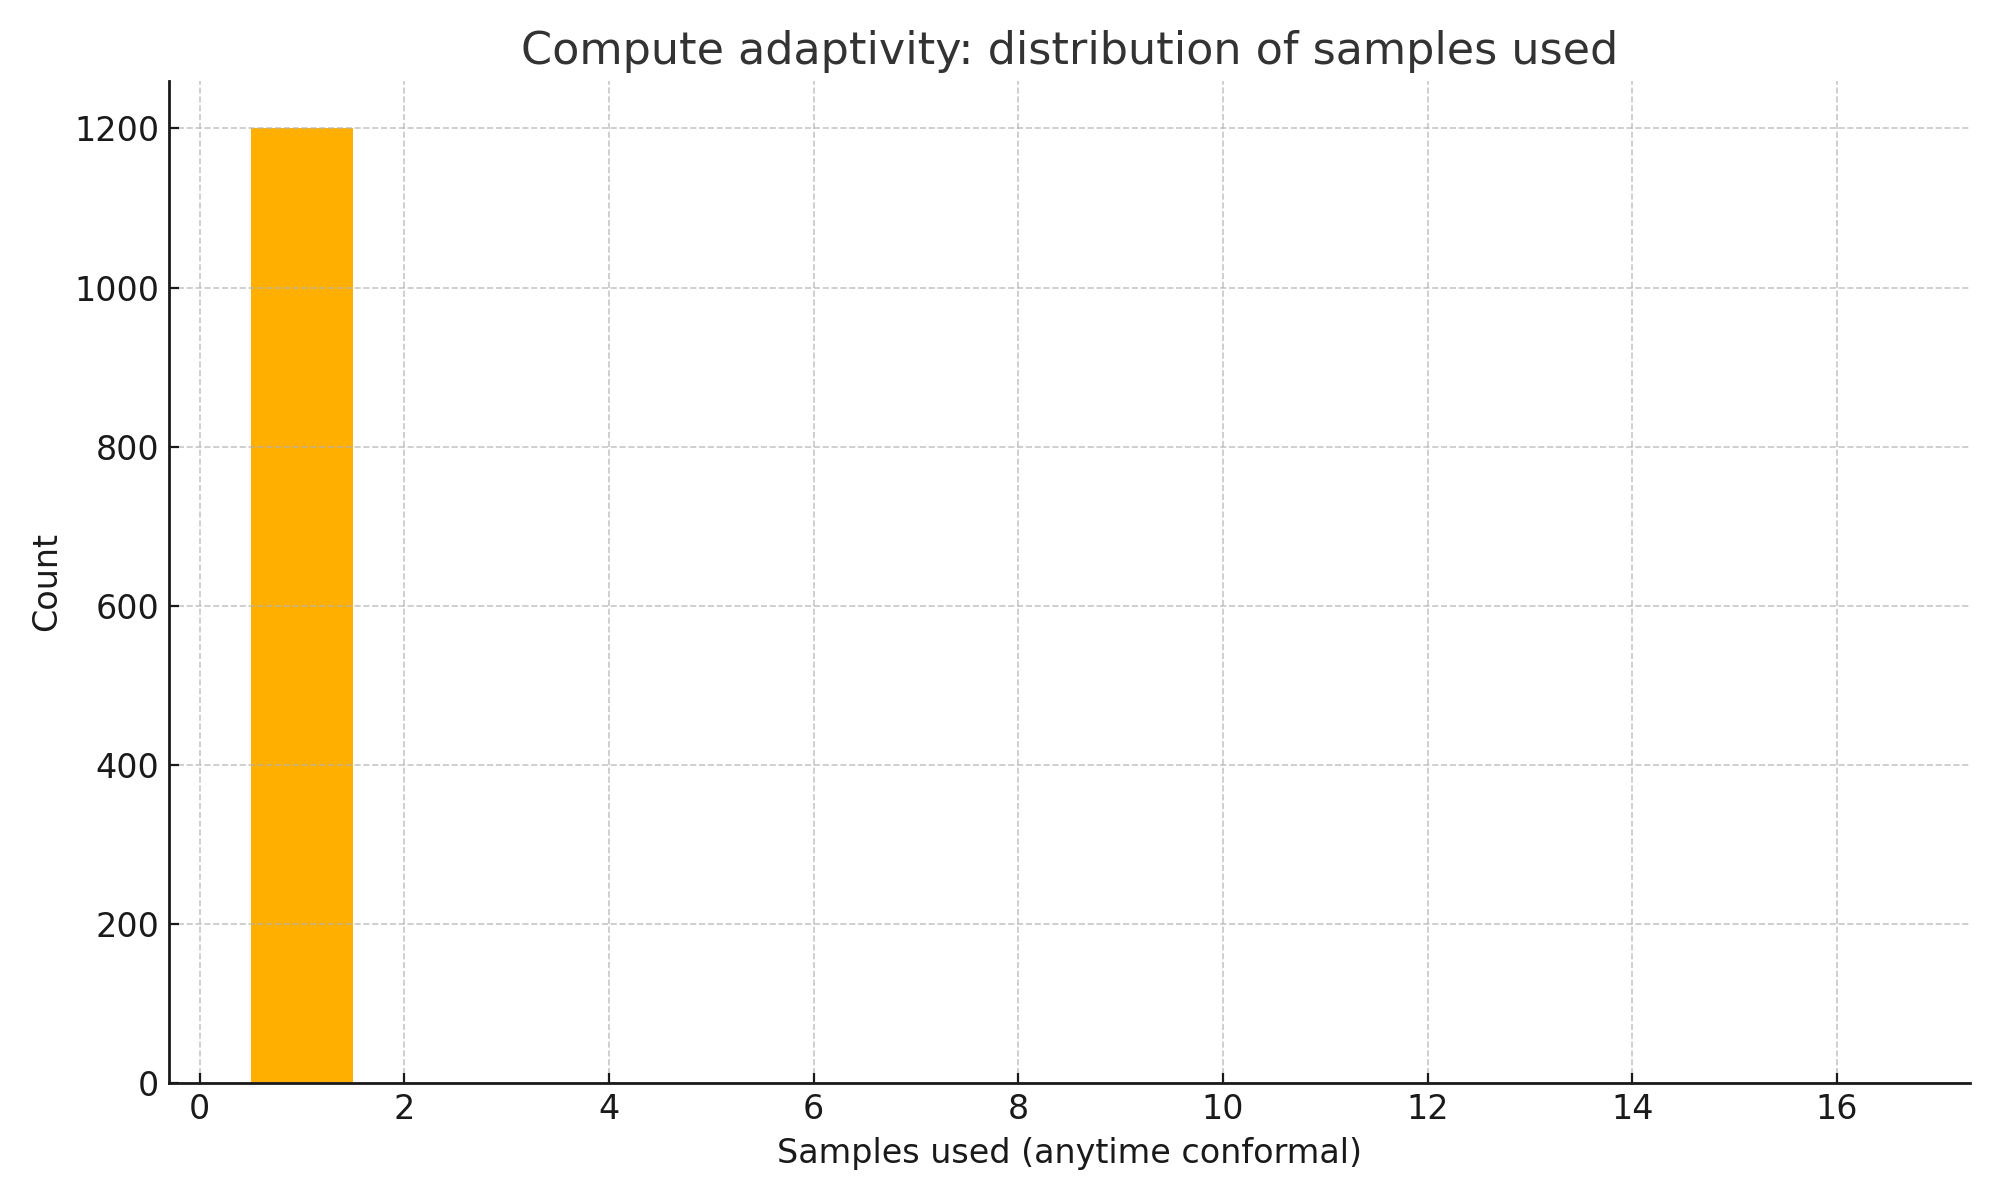
\includegraphics[width=0.6\textwidth]{samples_used_hist.png}
\caption{Distribution of samples used by ACSC (lower is cheaper), showing compute adaptivity across instances.}
\end{figure}

\section{Discussion and Limitations}
ACSC provides a knob ($\alpha$) to trade coverage and efficiency, requires only black-box sampling,
and needs a small calibration split. Guarantees are marginal and assume exchangeability between calibration
and test; domain shift can degrade coverage. Extending ACSC with class-conditional (Mondrian) calibration
and better nonconformity scores (e.g., combining vote-share with token-level log probabilities)
are promising directions.

\section{Conclusion}
We present ACSC, a training-free, compute-adaptive decoding method with coverage guarantees.
It is simple to implement, pairs naturally with self-consistency, and is suitable for low-compute deployments.

\paragraph{Reproducibility.} Code for our simulation and a minimal reference implementation are included in \texttt{simulation.py}.

\end{document}
